\documentclass[fleqn,11pt]{article}
\usepackage[utf8]{inputenc}
\usepackage[italian]{babel}

\usepackage{blindtext}
\usepackage{fancyhdr}
\usepackage{comment}

\usepackage{graphicx}
\graphicspath{ {./images/} }
\usepackage{wrapfig}

\usepackage{amsmath}
\usepackage{adjustbox}

\usepackage{listings}

\usepackage{tikz}
\usetikzlibrary{automata, positioning, arrows, arrows.meta}

\tikzset{
    ->, % makes the edges directed
    >=stealth, % makes the arrow heads bold
    -{Stealth[scale=1.1]},
    node distance=4.5cm, % specifies the minimum distance between two nodes. Change if necessary.
    every state/.style={align=center, very thick, fill=gray!10, minimum size=2cm}, % sets the properties for each ’state’ node
    initial text=$ $, % sets the text that appears on the start arrow
    every initial by arrow/.style={ultra thick},
}

%   MARGINS	  	  
\RequirePackage[left=1.5cm,%
right=1.5cm,%
top=2.0cm,%
bottom=2.0cm,%
headheight=14pt,%
a4paper]{geometry}%

\title{Progetto Finale di Reti Logiche}
\author{Giovanni Barbiero - 10722159}
\date{\today}

\makeatletter
\let\thetitle\@title
\let\theauthor\@author
\let\thedate\@date
\makeatother

\pagestyle{fancy}
\fancyhf{}
\rhead{\thedate}
\lhead{\thetitle}
\cfoot{\thepage}

\setlength{\parindent}{0pt}

\begin{document}

%   TITLE
{
    \hfill
    \begin{minipage}{0.2\textwidth}
        
\includegraphics[width=\linewidth]{logo}
    \end{minipage}
    \hfill
    \begin{minipage}{0.65\textwidth}
    \textsc{Terzo anno Ing. Informatica Politecnico di Milano}
    \end{minipage}
}
\\[0.4 cm]
\rule{\textwidth}{0.4pt}
{
    \LARGE
    \begin{center}
        \textbf{\thetitle}
    \end{center}
}
\begin{center}
    \Large
    \theauthor
\end{center}
\begin{center}
    \large
    \thedate
\end{center}


\section{Introduzione}
Lo scopo del progetto è quello di descrivere in linguaggio VHDL e di sintetizzare un componente hardware che legga i dati dalla memoria, effettui una codifica convoluzionale con rapporto \(\frac{1}{2}\) ed infine scriva il risultato in memoria.

\subsection{Descrizione generale}
La memoria da cui il componente legge e a cui scrive i dati è sincrona, a indirizzamento a byte e con uno spazio degli indirizzi a 16 bit. 
Il componente, servendosi della memoria, segue in ordine i seguenti passaggi:
\begin{enumerate}
    \item legge all'indirizzo di memoria \verb|0x0000| il numero di parole che dovrà codificare.
    \item partendo dall'indirizzo \verb|0x0001|, serializza le parole ottenendo una sequenza di bit.
    \item su questa sequenza applica la codifica convoluzionale \(\frac{1}{2}\) raddoppiando, così, il numero di bit.
    \item la nuova sequenza di bit viene infine scritta in memoria a partire dall'indirizzo \verb|0x03E8|.
\end{enumerate}
La sequenza di parole da codificare è al massimo di 255, inoltre il componente deve funzionare correttamente con un periodo di clock di almeno \verb|100 ns|.  

\subsection{Codifica convoluzionale}
Il codificatore convoluzionale con tasso di trasmissione \(\frac{1}{2}\) è un componente che per ogni bit che riceve in ingresso genera la sua codifica in 2 bit.
Si può rappresentare come una macchina a stati di Mealy con un bit per l'ingresso e 2 bit per l'uscita come in Figura \ref{fig:codconv}.

\begin{figure}[b]
    \centering
    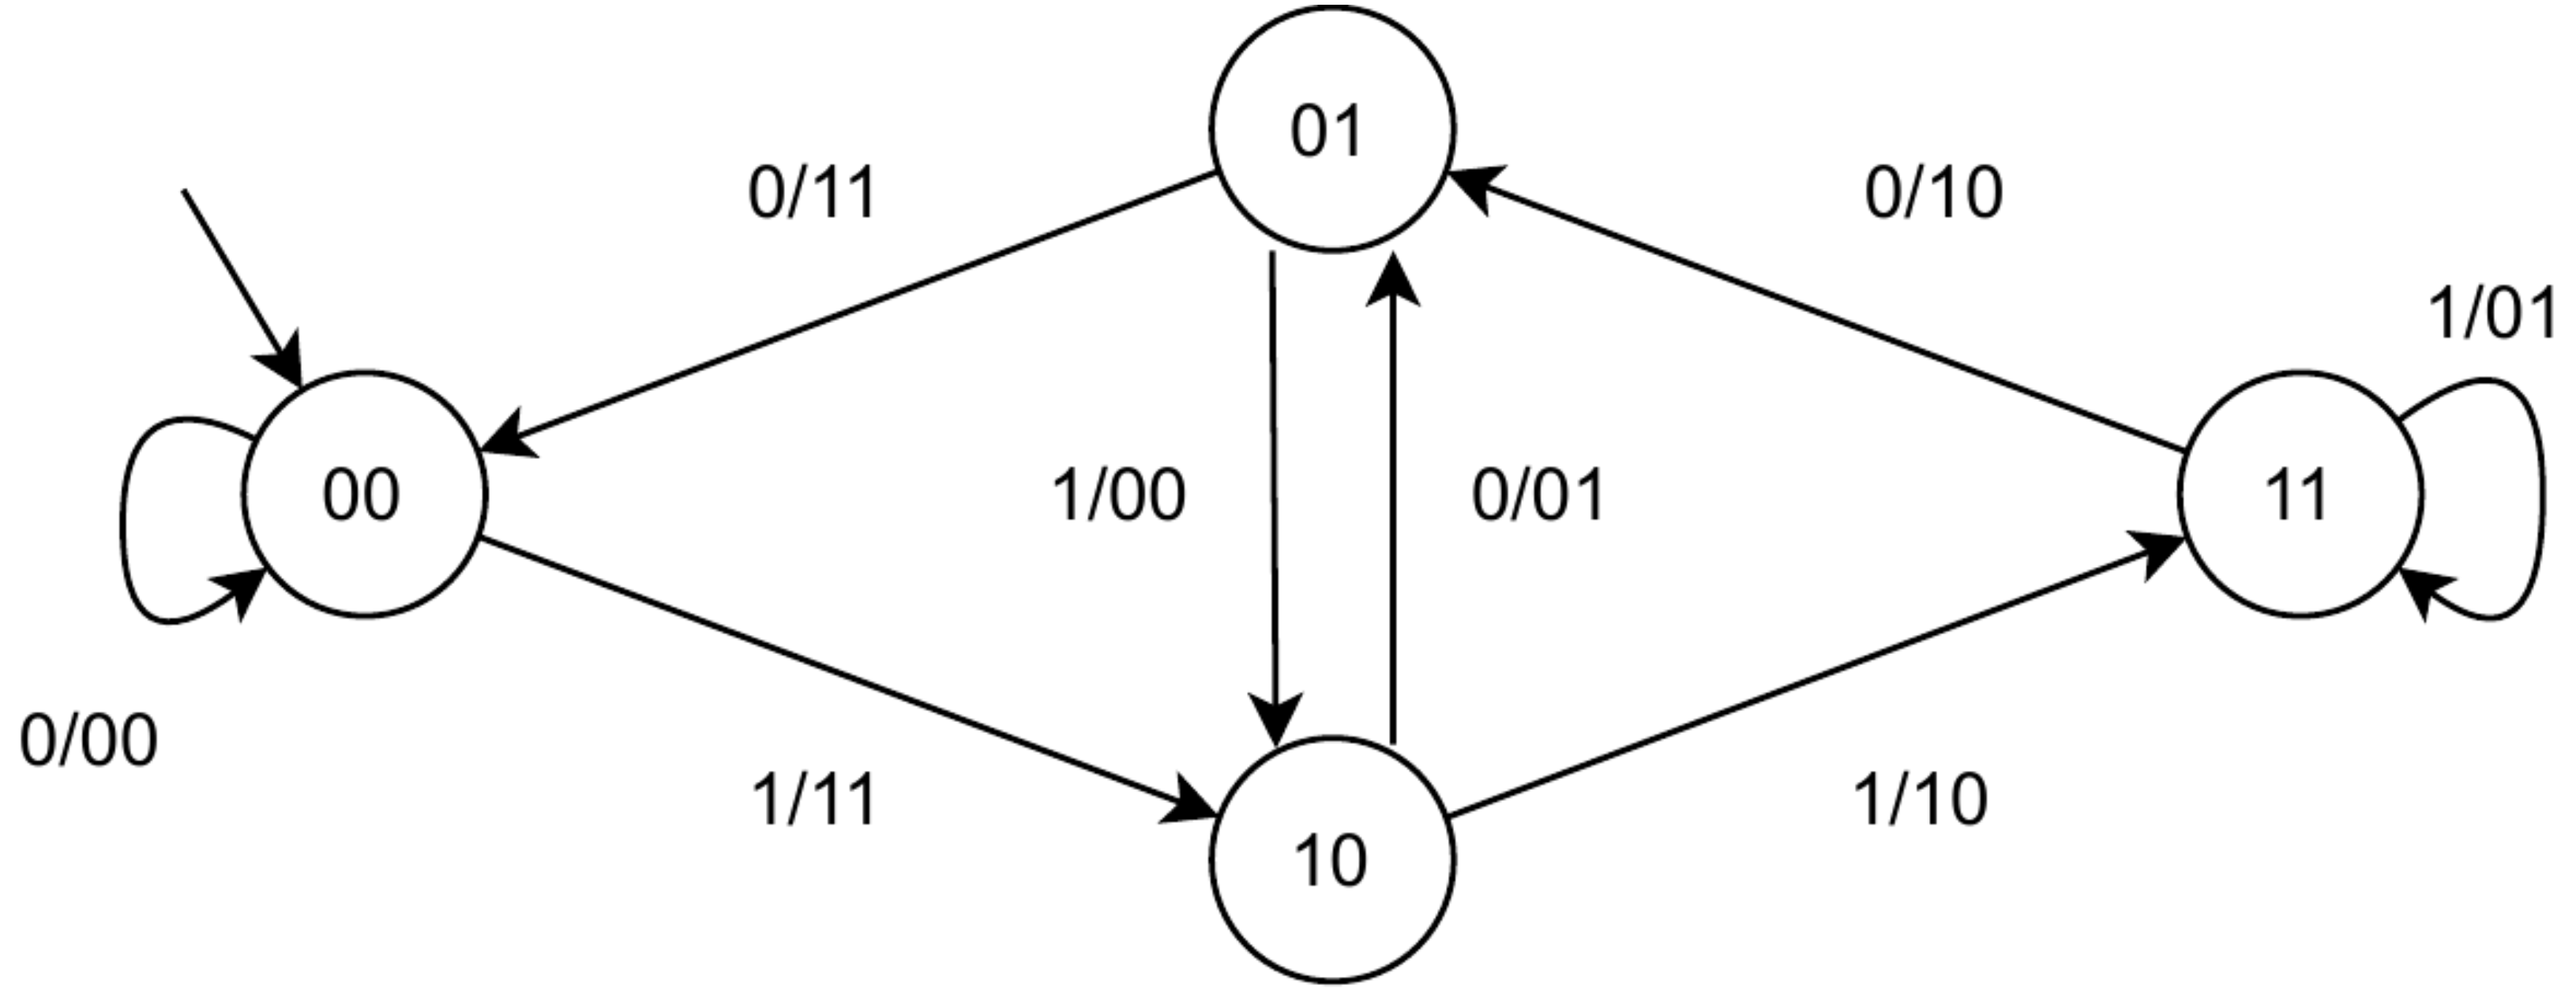
\includegraphics[width=0.75\textwidth]{codconv}
    \caption{Codifica convoluzionale con rapporto \(\frac{1}{2}\).}
    \label{fig:codconv}
\end{figure}

\subsection{Esempio di funzionamento}
Il componente legge dalla memoria (Tabella \ref{tab:memIniz}) all'indirizzo \verb|0x0000| il numero di parole totale da codificare.
Successivamente partendo dall'indirizzo \verb|0x0001| legge la prima parola, la quale viene serializzata e il singolo bit viene dato in ingresso al codificatore convoluzionale come in Tabella \ref{tab:conv}.
Quest'ultimo produce due bit in ogni istante \verb|t|, i quali vengono deserializzati e scritti in memoria a partire dall'indirizzo \verb|0x03E8|.\\
Una volta codificata la prima parola il codificatore continua con le successive fino ad averle codificate tutte.\\
Il contenuto della memoria alla fine della codifica è riportato in Tabella \ref{tab:memFin}.\\

\begin{table}[h]
    \begin{minipage}{0.45\textwidth}
        \centering
        \begin{tabular}{|c|c|}
            \hline
            Indirizzo & Contenuto \\
            \hline
            \verb|0x0000| & \verb|00000010| \\ 
            \verb|0x0001| & \verb|10100010| \\ 
            \verb|0x0002| & \verb|01001011| \\ 
            \hline
        \end{tabular}
        \caption{Contenuto iniziale memoria.}
        \label{tab:memIniz}
    \end{minipage}
    \hfill
    \begin{minipage}{0.45\textwidth}
        \centering
        \begin{tabular}{|c|c|}
            \hline
            Indirizzo & Contenuto \\
            \hline
            \verb|0x03E8| & \verb|11010001| \\ 
            \verb|0x03E9| & \verb|11001101| \\ 
            \verb|0x03EA| & \verb|11110111| \\ 
            \verb|0x03EB| & \verb|11010010| \\ 
            \hline
        \end{tabular}
        \caption{Contenuto finale memoria.}
        \label{tab:memFin}
    \end{minipage}
\end{table}

\begin{table}[h]
    \centering
    \begin{tabular}{|c|c c c c c c c c|}
        \hline
        \verb|t| & 0 & 1 & 2 & 3 & 4 & 5 & 6 & 7 \\
        \hline
        \verb|in| & 1 & 0 & 1 & 0 & 0 & 0 & 1 & 0 \\
        \verb|out_1| & 1 & 0 & 0 & 0 & 1 & 0 & 1 & 0 \\
        \verb|out_2| & 1 & 1 & 0 & 1 & 1 & 0 & 1 & 1 \\
        \hline
        \hline
        \verb|t| & 8 & 9 & 10 & 11 & 12 & 13 & 14 & 15 \\
        \hline
        \verb|in| & 0 & 1 & 0 & 0 & 1 & 0 & 1 & 1 \\
        \verb|out_1| & 1 & 1 & 0 & 1 & 1 & 0 & 0 & 1 \\
        \verb|out_2| & 1 & 1 & 1 & 1 & 1 & 1 & 0 & 0 \\
        \hline
    \end{tabular}
    \caption{Codifica convoluzionale al tempo t.}
    \label{tab:conv}
\end{table}

\section{Architettura}
Il componente possiede la seguente interfaccia:
\begin{lstlisting}[language=VHDL]
entity project_reti_logiche is
    port (
        i_clk     : in  std_logic;
        i_rst     : in  std_logic;
        i_start   : in  std_logic;
        i_data    : in  std_logic_vector(7  downto 0);
        o_address : out std_logic_vector(15 downto 0);
        o_done    : out std_logic;
        o_en      : out std_logic;
        o_we      : out std_logic;
        o_data    : out std_logic_vector (7  downto 0)
    );
end project_reti_logiche;
\end{lstlisting}
L'elaborazione inizia quando viene alzato il segnale \verb|i_start| e termina quando il componente alza il segnale \verb|o_done|. Solo successivamente il segnale \verb|i_start| dovrà essere abbassato.\\
Il componente è stato strutturato in vari moduli e in una macchina a stati che ne coordina l'interoperabilità al fine di ottenere un corretto funzionamento secondo le specifiche.
In Figura \ref{fig:modgen} si può osservare come i moduli sono connessi tra loro. A tutti i moduli, compresa la macchina a stati, vengono forniti il segnale di clock \verb|i_clk| e il segnale di reset \verb|i_rst|.
%In seguito vengono descritti i vari moduli e la macchina a stati.

\begin{figure}
    \centering
    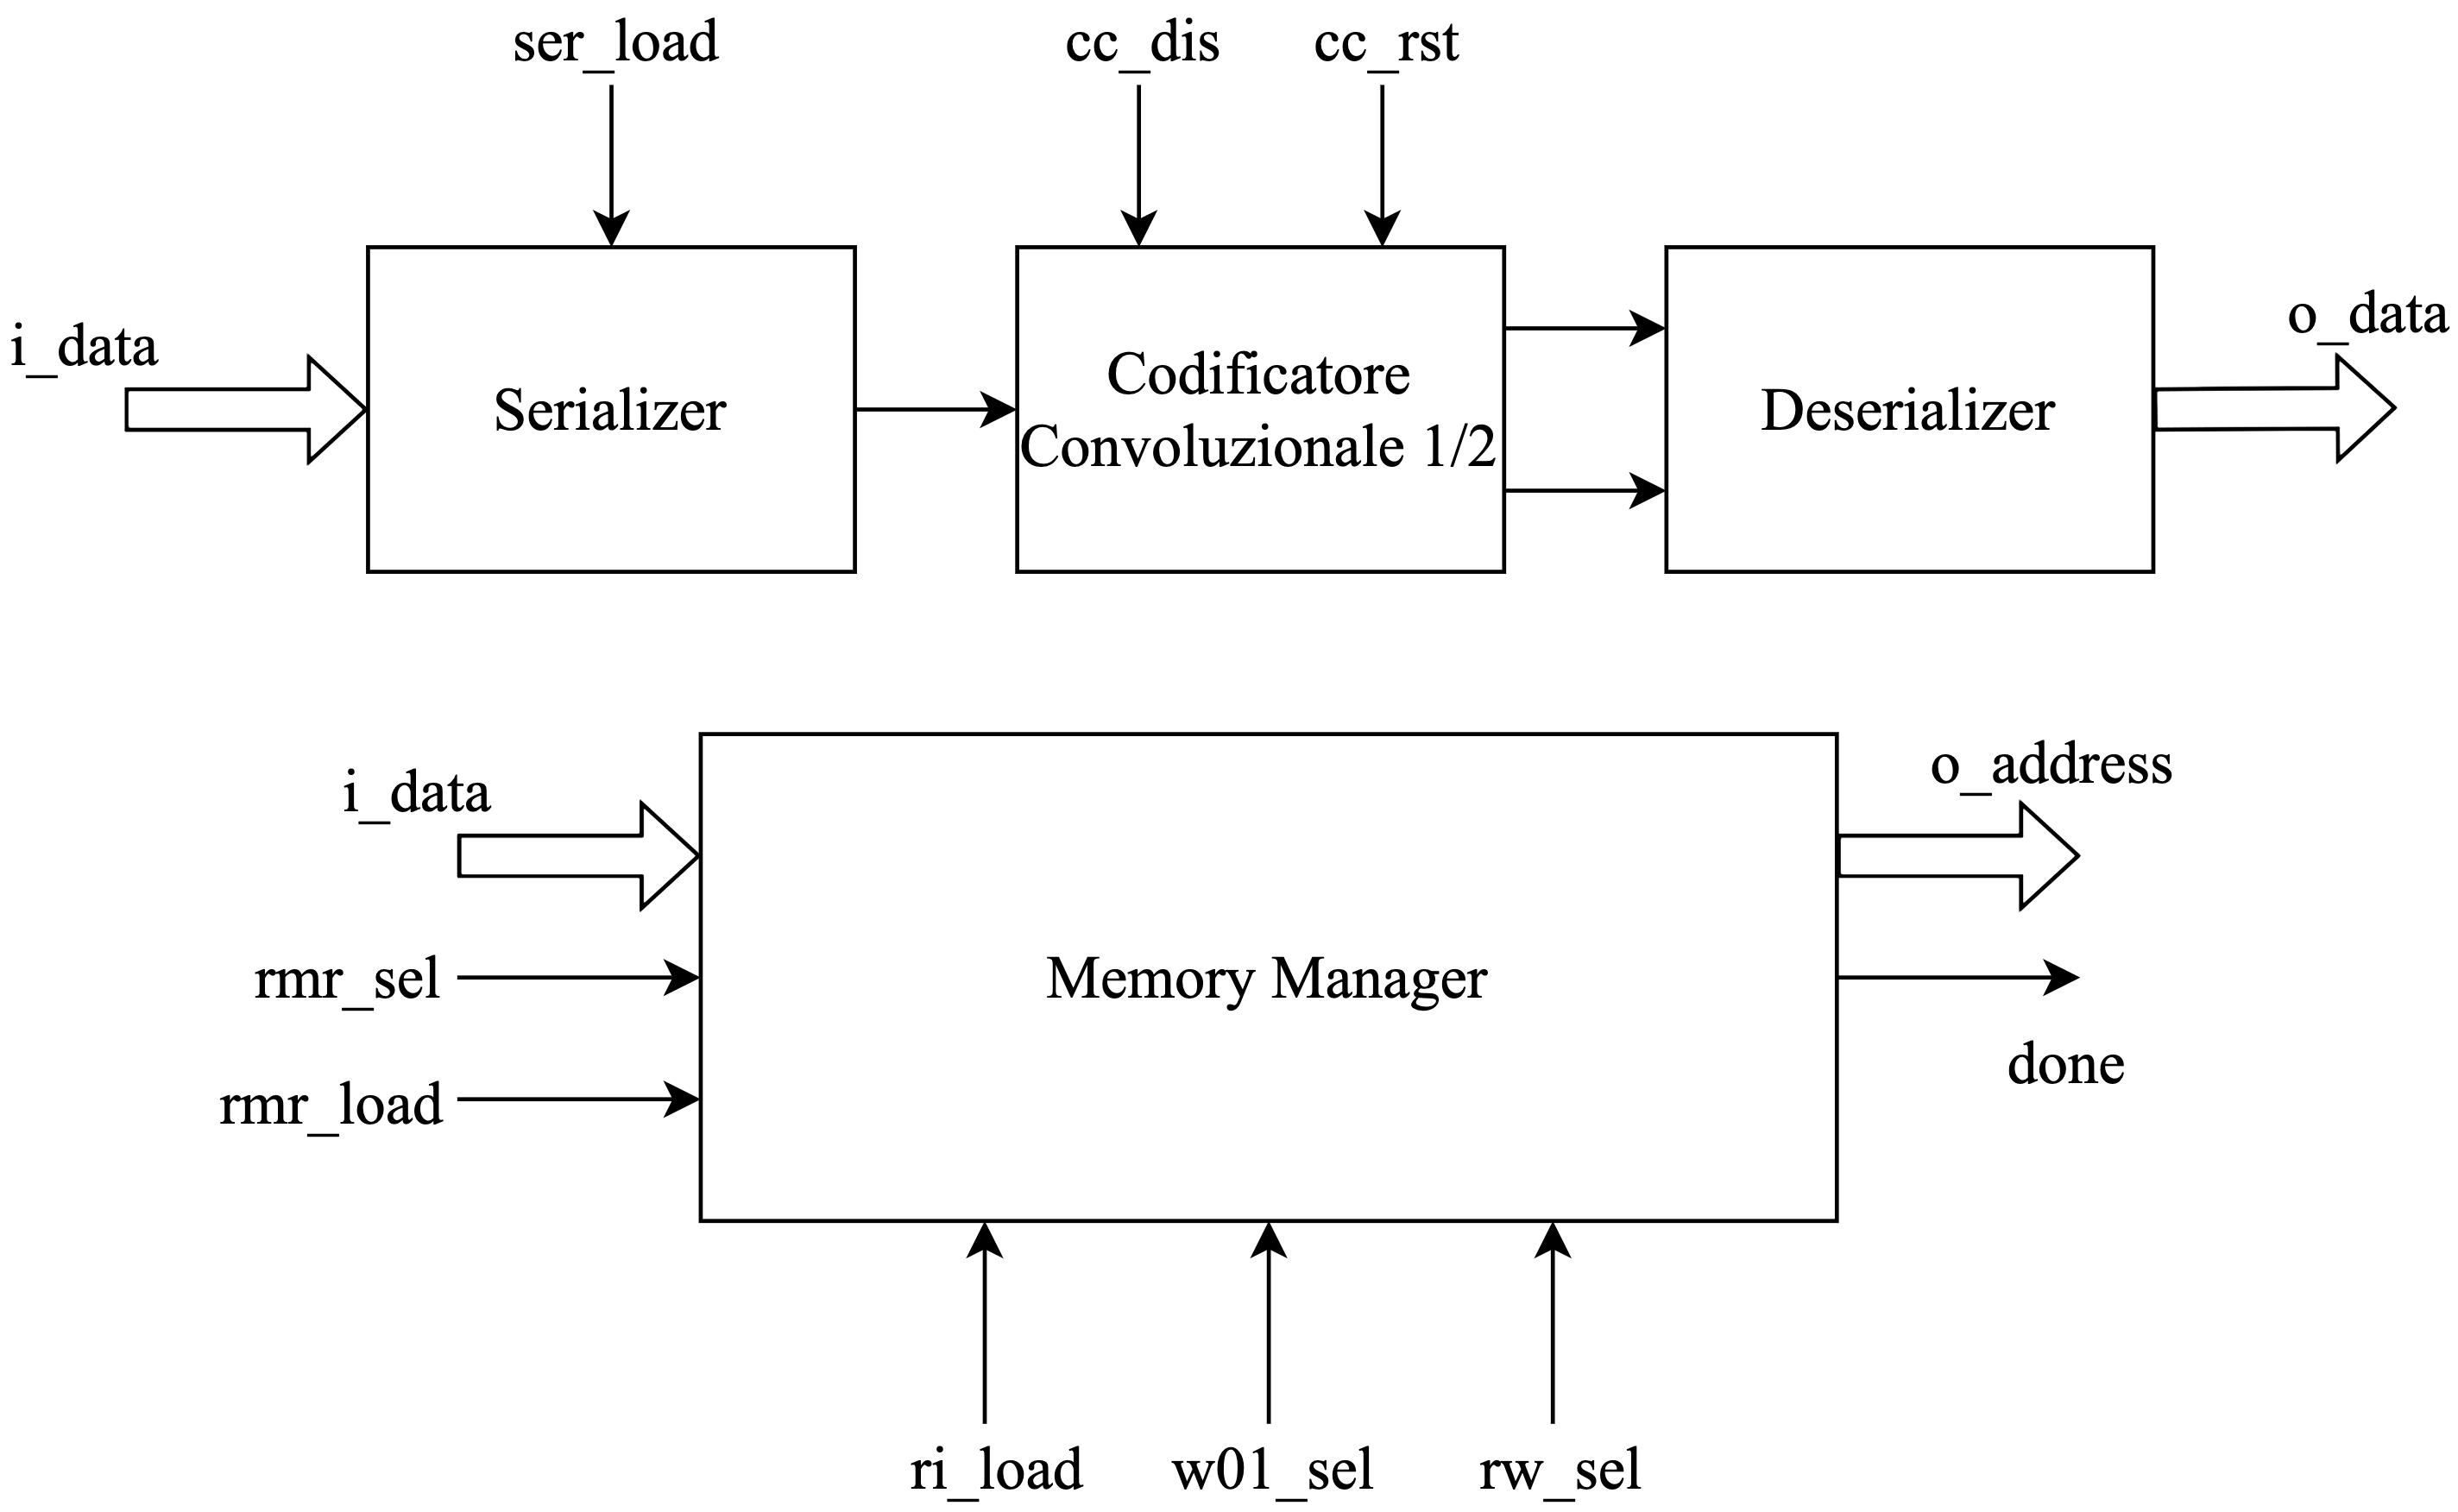
\includegraphics[width=0.6\textwidth]{module_connections}
    \caption{Connessioni tra i moduli.}
    \label{fig:modgen}
\end{figure}

\begin{figure}
    \centering
    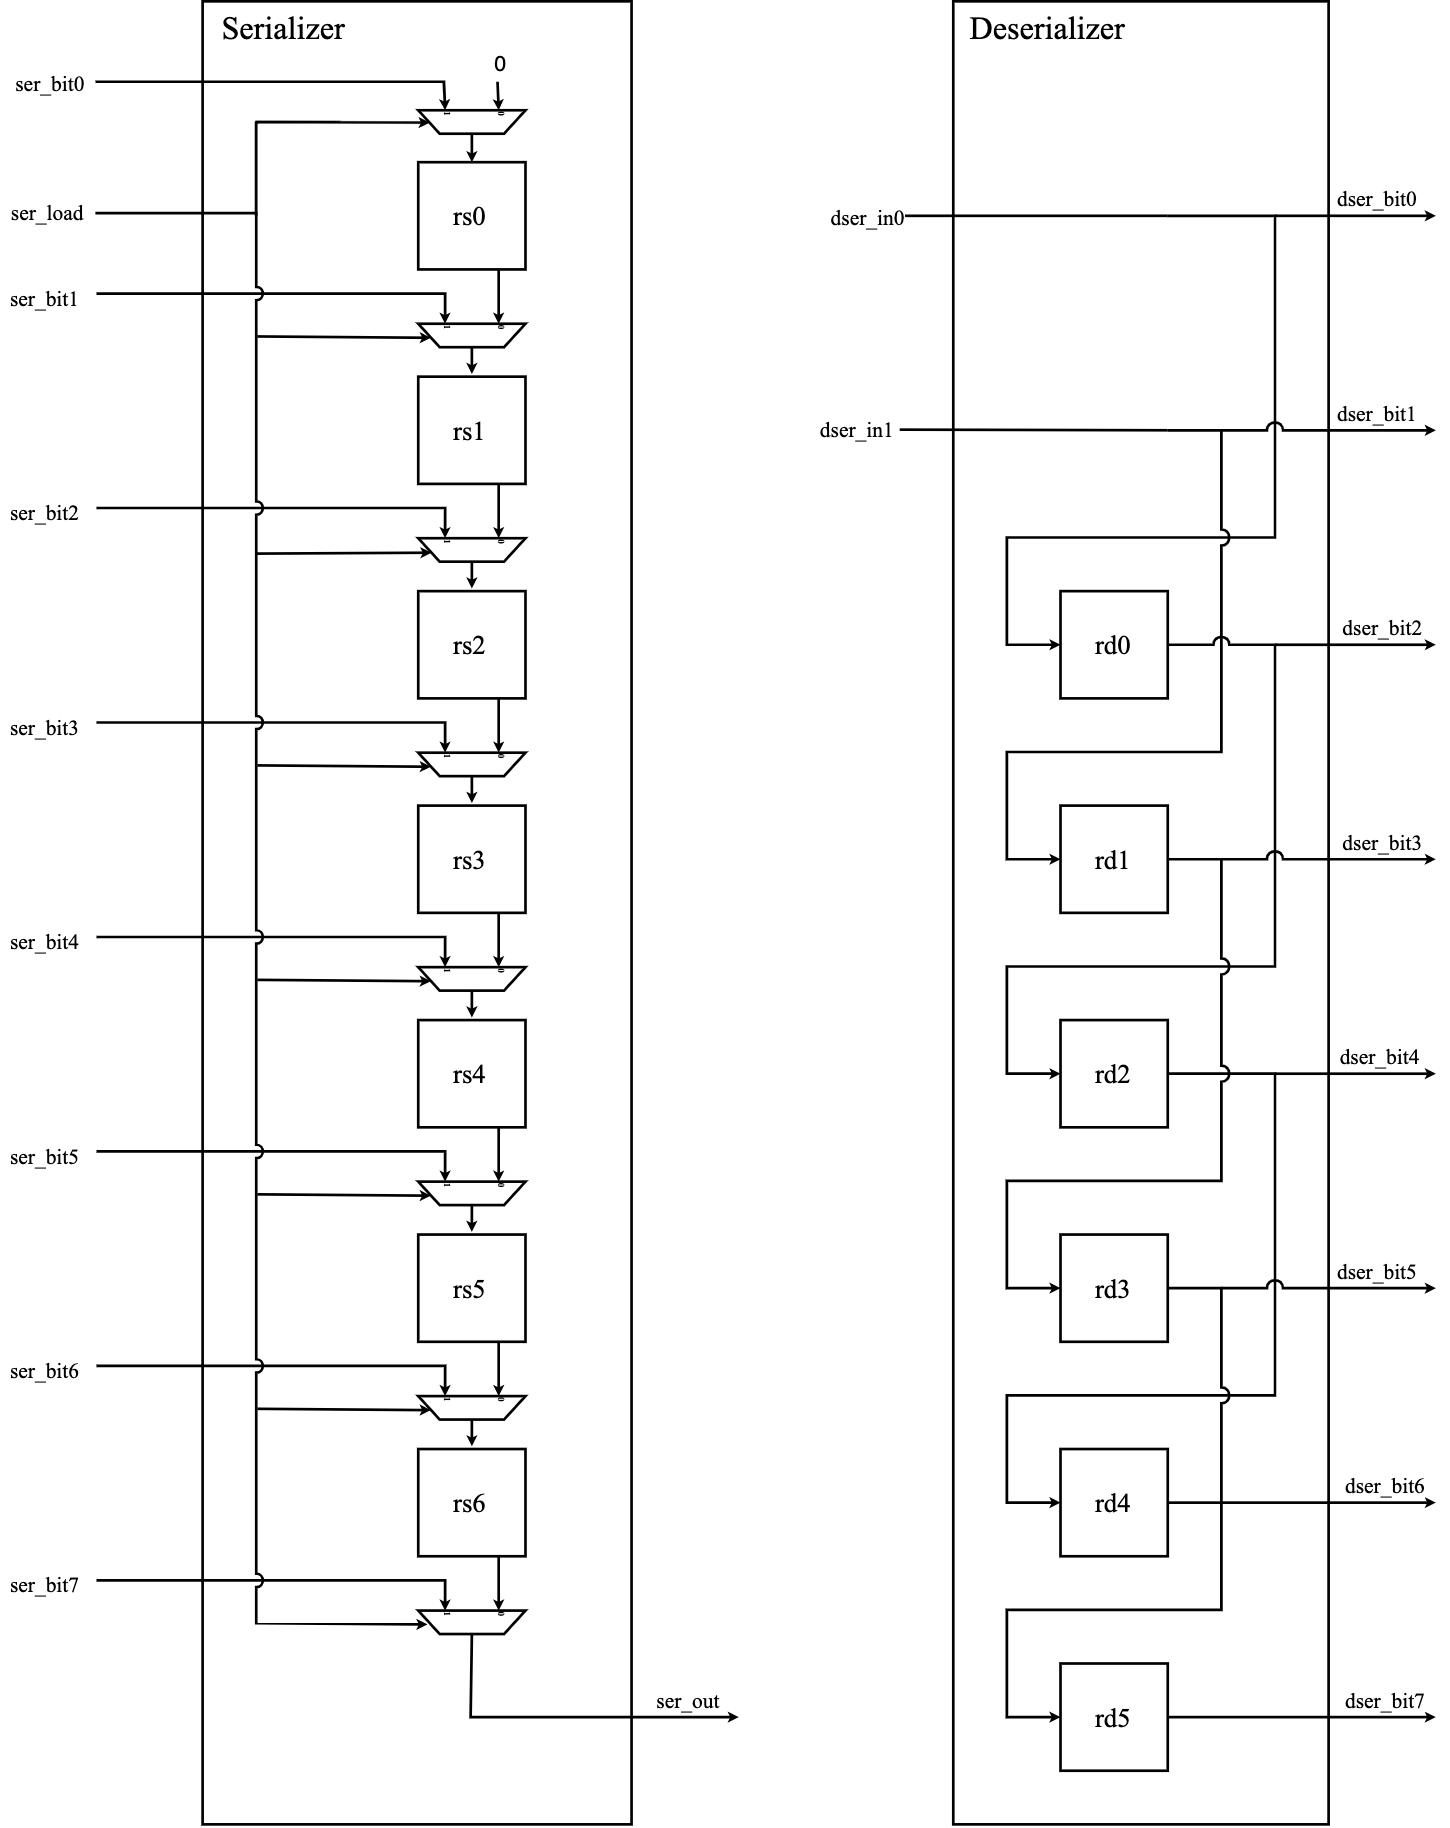
\includegraphics[height=0.7\textwidth]{ser_deser}
    \caption{Schema implementativo di serializzatore e deserializzatore.}
    \label{fig:ser_deser}
\end{figure}

\subsection{Serializzatore}
Il serializzatore riceve in ingresso i dati dalla memoria in \verb|i_data| e seguendo il segnale di clock mette in uscita un bit alla volta i dati letti partendo dal più significativo.\\
Come mostrato in modo dettagliato in Figura \ref{fig:ser_deser}, il serializzatore è un registro a scorrimento di tipo PISO (parallel input-serial output) a 8 bit dove l'ultimo flip flop è stato rimosso per risparmiare un ciclo di clock. 
Quando il segnale \verb|ser_load = 1| viene memorizzato \verb|i_data|, altrimenti viene effettuato lo shift.

\subsection{Deserializzatore}
Il deserializzatore riceve in ingresso due bit \verb|dser_in0| e \verb|dser_in1| e seguendo il segnale di clock appende ai bit presenti i due nuovi bit.\\
Come mostrato in modo dettagliato in Figura \ref{fig:ser_deser}, il deserializzatore è un registro a scorrimento di tipo SIPO (serial input-parallel output) a 8 bit con uno shift di 2 bit alla volta e i primi due flip flop rimossi per risparmiare un ciclo di clock.\\
L'uscita del deserializzatore viene poi direttamente collegata ad \verb|o_data| per poter essere scritta in memoria quando i segnali \verb|o_en| e \verb|o_we| vengono alzati.

\subsection{Codificatore convoluzionale}
Il codificatore convoluzionale con rapporto \(\frac{1}{2}\) è l'implementazione della macchina a stati in Figura \ref{fig:codconv}.\\
Il segnale \verb|cc_dis| serve per bloccare l'avanzamento della macchina a stati, mentre il segnale \verb|cc_rst| per resettare la macchina a stati e portarla allo stato iniziale \verb|00|. Questo risulta l'unico modulo ad essere scollegato dal segnale \verb|i_rst|, però, come verrà mostrato in seguito, quando la macchina a stati si trova nello stato di reset allora alza il segnale \verb|cc_rst| resettando così anche il codificatore convoluzionale.

\begin{figure}[h]
    \centering
    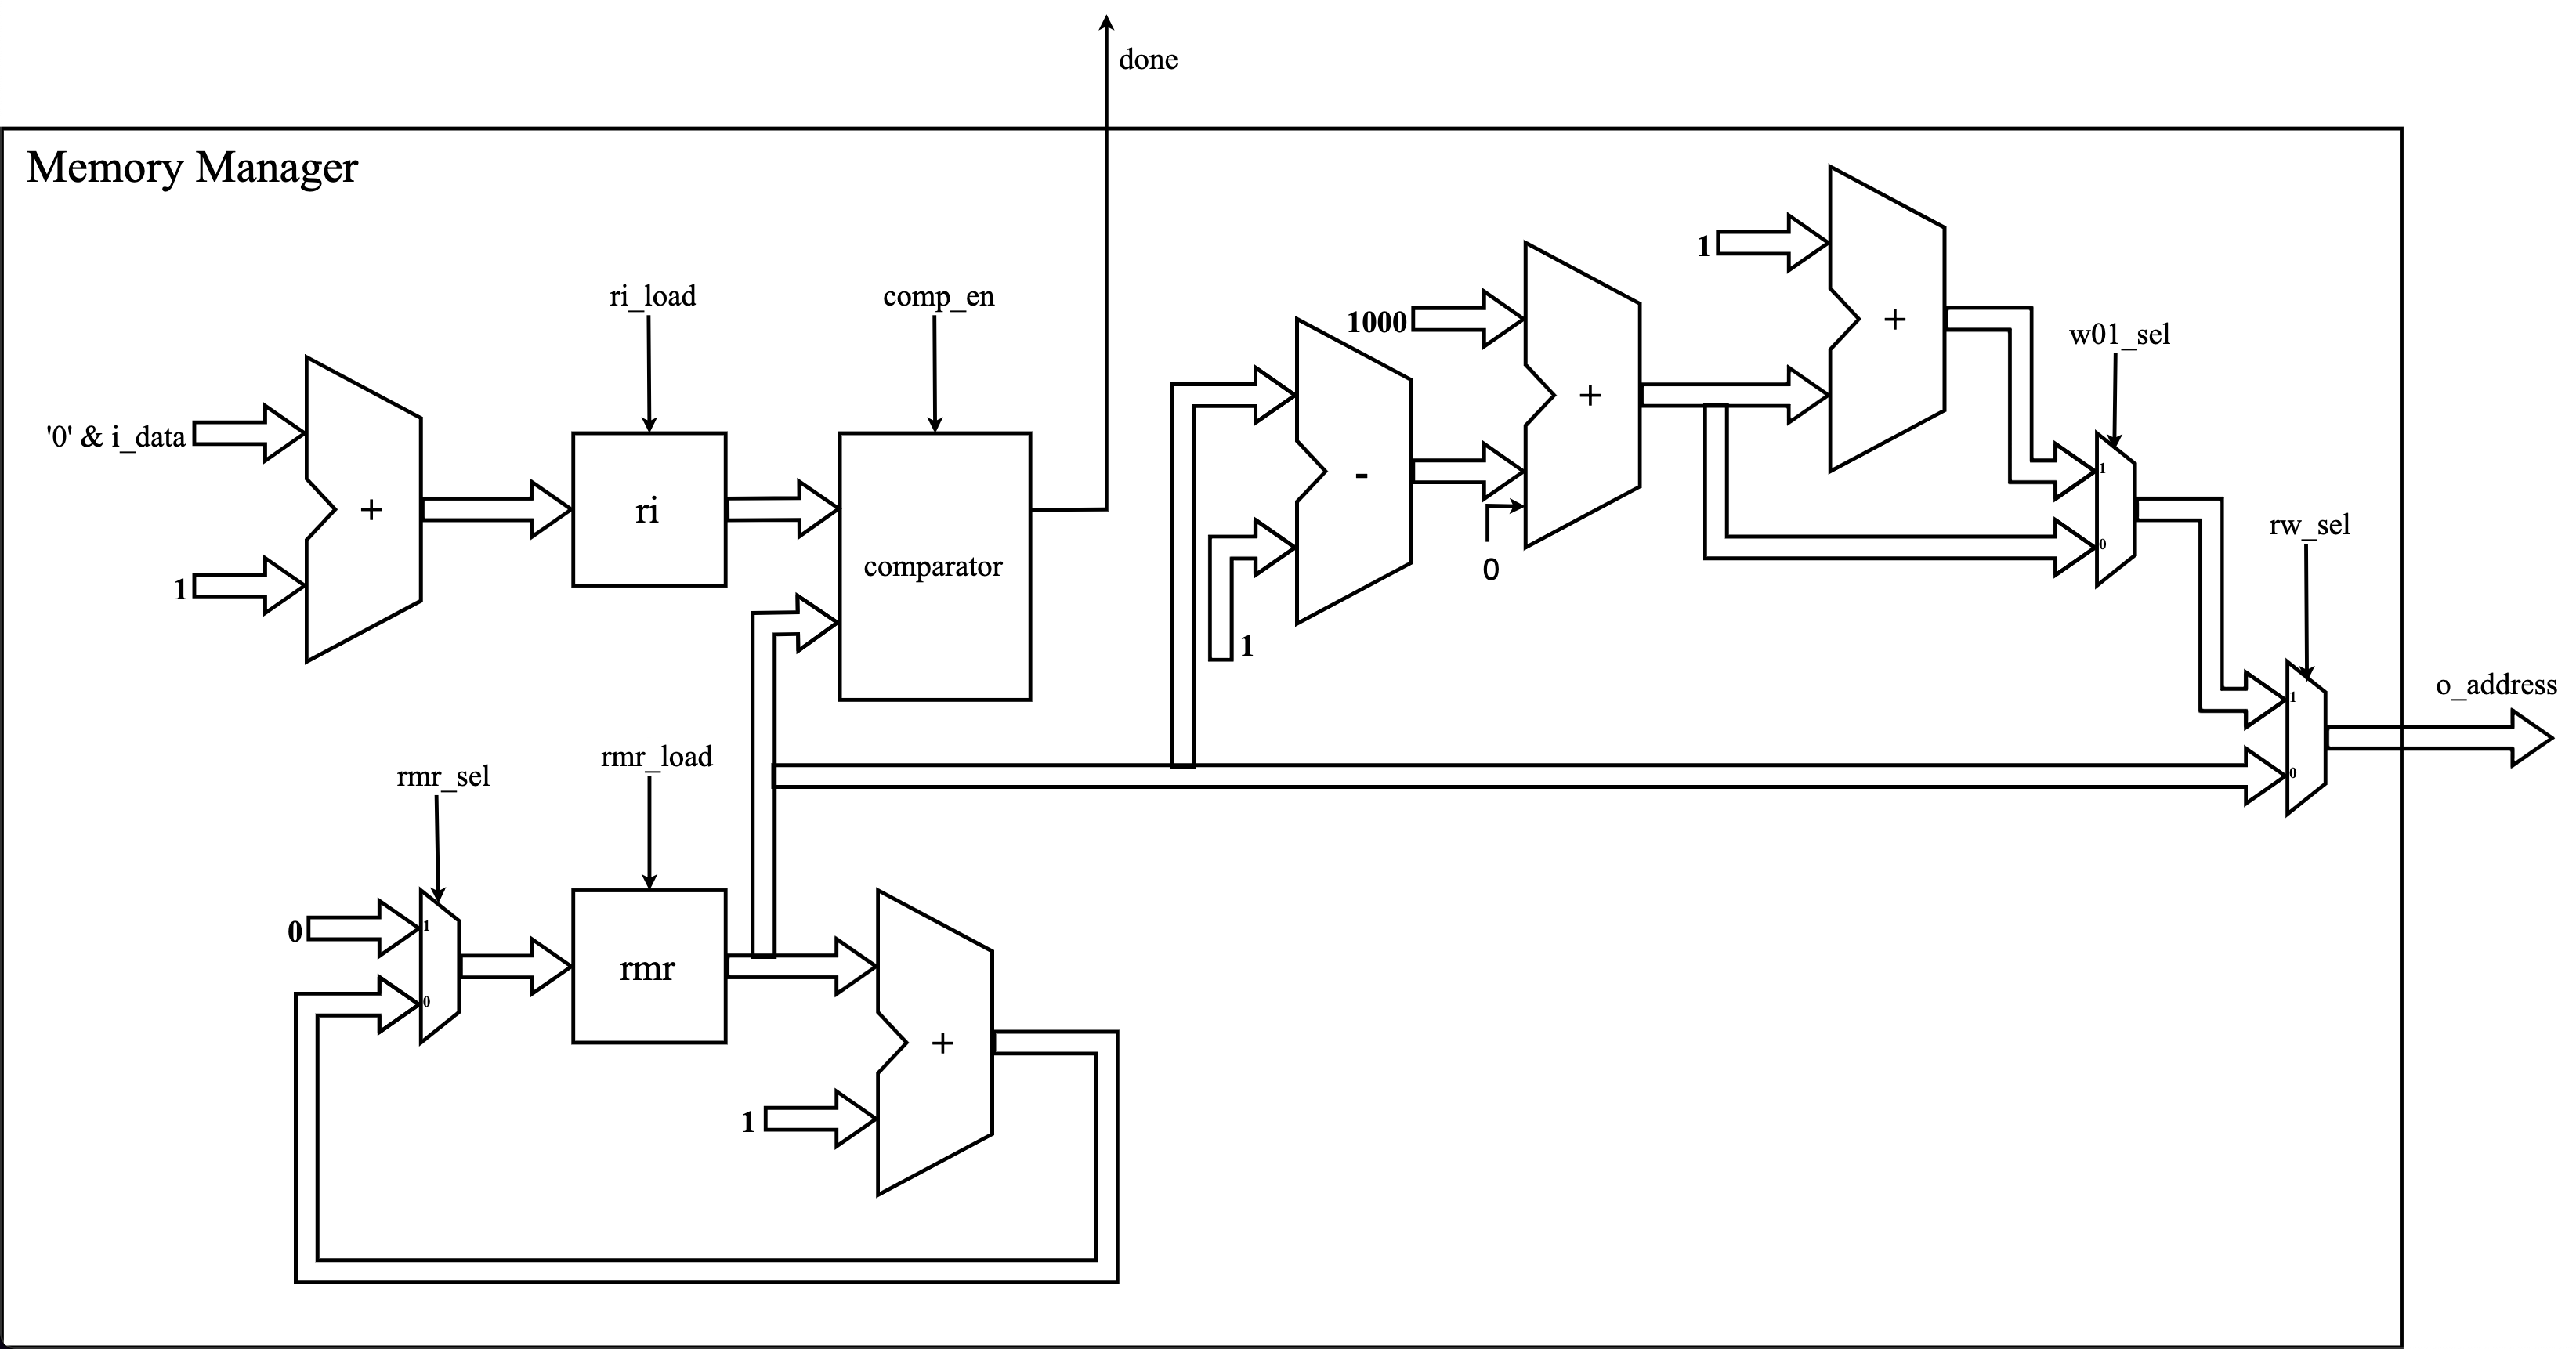
\includegraphics[width=\textwidth]{mem_manager}
    \caption{Struttura interna del gestore della memoria.}
    \label{fig:mem_man}
\end{figure}

\subsection{Gestore della memoria}
Il gestore della memoria ha il compito di tener traccia di quante parole devono essere lette e gestire gli indirizzi di memoria sia per la lettura che per la scrittura.\\
La struttura interna viene mostrata in Figura \ref{fig:mem_man}.\\
Tramite il segnale \verb|ri_load| viene salvato il numero di parole totale da leggere $+ 1$ nel registro \verb|ri| a 9 bit.
Nel registro \verb|rmr| viene salvato l'indirizzo della parola corrente e tramite il segnale \verb|rmr_load| ne viene aggiornato il valore. Quest'ultimo in base a \verb|rmr_sel| può essere il valore precedente incrementato di uno oppure \verb|0|.
Il segnale \verb|rmr_sel| viene utilizzato per questo scopo, cioè di riportare il contatore a zero per poter consentire la codifica di nuovi flussi senza reset.\\
Dato che per ogni parola letta se ne scrivono due, si può calcolare l'indirizzo dove scrivere il risultato della codifica come \(\verb|0x03E8| + 2\cdot\verb|n|\) e \(\verb|0x03E8| + 2\cdot\verb|n| + 1\) dove \verb|n| corrisponde al valore del registro \verb|rmr|.\\
Il segnale \verb|w01_sel| serve per selezionare in quale tra i due indirizzi scrivere il risultato della codifica, mentre il segnale \verb|rw_sel| serve per selezionare tra gli indirizzi di lettura e quelli di scrittura.\\
Inoltre, in modo asincrono, viene effettuato il confronto tra i valori dei registri \verb|ri| e \verb|rmr|. Se questi ultimi coincidono significa che sono state lette tutte le parole, quindi il segnale interno \verb|done| viene portare a \verb|1|.\\
I registri \verb|ri| e \verb|rmr| sono a 9 bit poiché le parole massime che il componente deve poter codificare sono 255 che richiede almeno 9 bit per essere codificato in binario.

\subsection{Macchina a stati}
La macchina a stati (vedi Figura \ref{fig:fsm}) ha lo scopo di gestire i segnali di comando in input al componente e di modificare i segnali interni per consentire la corretta interoperabilità dei vari moduli.\\
È una macchina a stati di Moore ed è formata dai seguenti stati:
\begin{itemize}
    \item \verb|IDLE|: Stato iniziale in cui si resetta sia il contatore degli indirizzi di memoria sia il codificatore convoluzionale. Inoltre questo stato rappresenta anche lo stato di reset della macchina.
    \item \verb|READ_0|: Quando viene alzato il segnale \verb|i_start| si arriva in questo stato. Viene richiesto alla memoria il contenuto all'indirizzo \verb|0x0000| e il codificatore convoluzionale viene disabilitato.
    \item \verb|SAVE|: In questo stato viene salvato il valore che arriva dalla memoria nel registro \verb|ri| e il codificatore rimane disabilitato.
    \item \verb|READ_I|: Si richiede alla memoria il contenuto dell'indirizzo salvato nel registro \verb|rmr| e si continua a tener disabilitato il codificatore convoluzionale.
    \item \verb|COMP_00|: Viene caricata la parola nel serializzatore e il codificatore convoluzionale, ora abilitato, ne codifica il primo bit.
    \item \verb|COMP_01|: Passaggio intermedio di codifica della parola: viene codificato il secondo bit.
    \item \verb|COMP_02|: Passaggio intermedio di codifica della parola: viene codificato il terzo bit.
    \item \verb|WRITE_0|: Passaggio intermedio di codifica della parola: viene codificato il quarto bit. Inoltre la codifica della prima metà della parola viene scritta in memoria all'indirizzo \(\verb|0x03E8| + 2\cdot\verb|rmr|\).
    \item \verb|COMP_10|: Passaggio intermedio di codifica della parola: viene codificato il quinto bit.
    \item \verb|COMP_11|: Passaggio intermedio di codifica della parola: viene codificato il sesto bit.
    \item \verb|COMP_12|: Passaggio intermedio di codifica della parola: viene codificato il settimo bit.
    \item \verb|WRITE_1|: Ultimo passaggio di codifica della parola: viene codificato l'ottavo bit. Inoltre la codifica della seconda metà della parola viene scritta in memoria all'indirizzo \(\verb|0x03E8| + 2\cdot\verb|rmr| + 1\).
    \item \verb|WAIT_S|: Se la macchina a stati si trova nello stato di \verb|READ_I| e il segnale \verb|done| è alto allora si arriva in questo stato. Si continua a rimanere in questo stato con \verb|o_done = 1| fintanto che \verb|i_start| rimane alzato. Quando \verb|i_start| viene abbassato la macchina a stati si porta nello stato \verb|IDLE|.
\end{itemize}

\pagebreak
\null
\vfill
\begin{figure}[h]
    \centering
    \begin{tikzpicture}
        \node[state, initial, accepting, initial distance=1cm, align=center] (s0) {\texttt{IDLE}};
        \node[state, right of=s0] (s1) {\verb|READ_0|};
        \node[state, right of=s1] (s2) {\verb|SAVE|};
        \node[state, right of=s2] (s3) {\verb|READ_I|};
        \node[state, below of=s3] (s4) {\verb|COMP_00|};
        \node[state, below of=s2] (s5) {\verb|COMP_01|};
        \node[state, below of=s1] (s6) {\verb|COMP_02|};
        \node[state, below of=s0] (s7) {\verb|WRITE_0|};
        \node[state, below of=s7] (s8) {\verb|COMP_10|};
        \node[state, below of=s6] (s9) {\verb|COMP_11|};
        \node[state, below of=s5] (s10) {\verb|COMP_12|};
        \node[state, below of=s4] (s11) {\verb|WRITE_1|};
        \node[state, above of=s1, xshift=2.25cm, yshift=-2cm] (s12) {\verb|WAIT_S|};
        
        \node[rectangle, align=center, below=0.1cm of s0] (s0-below) {
            {\small \verb|rmr_sel = 1|} \\
            {\small \verb|rmr_load = 1|} \\
            {\small \verb|cc_dis = 1|} \\
            {\small \verb|cc_rst = 1|}
        };
        \node[rectangle, align=center, below=0.1cm of s1] (s1-below) {
            {\small \verb|o_en = 1|} \\
            {\small \verb|rmr_load = 1|} \\
            {\small \verb|cc_dis = 1|}
        };
        \node[rectangle, align=center, below=0.1cm of s2] (s2-below) {
            {\small \verb|ri_load = 1|} \\
            {\small \verb|cc_dis = 1|}
        };
        \node[rectangle, align=center, below=0.1cm of s3] (s3-below) {
            {\small \verb|o_en = 1|} \\
            {\small \verb|cc_dis = 1|}
        };
        \node[rectangle, align=center, below=0.1cm of s4] (s4-below) {
            {\small \verb|ser_load = 1|}
        };
        \node[rectangle, align=center, below=0.1cm of s7] (s7-below) {
            {\small \verb|o_en = 1|} \\
            {\small \verb|o_we = 1|} \\
            {\small \verb|rw_sel = 1|}
        };
        \node[rectangle, align=center, below=0.1cm of s11] (s11-below) {
            {\small \verb|o_en = 1|} \\
            {\small \verb|o_we = 1|} \\
            {\small \verb|w01_sel = 1|} \\
            {\small \verb|rw_sel = 1|} \\
            {\small \verb|rmr_load = 1|}
        };
        \node[rectangle, align=center, below=0.1cm of s12] (s12-below) {
            {\small \verb|o_done = 1|}
        };
        
        \draw[ultra thick] (s0) edge[loop above] node{\texttt{i\_start = 0}} (s0);
        \draw[very thick] (s0) edge[below] node{\texttt{i\_start = 1}} (s1);
        \draw[very thick] (s1) -- (s2);
        \draw[very thick] (s2) -- (s3);
        \draw[very thick] (s3) edge[bend right=45] node[sloped, anchor=center, below]{\texttt{done = 0}} (s4);
        \draw[very thick] (s4) -- (s5);
        \draw[very thick] (s5) -- (s6);
        \draw[very thick] (s6) -- (s7);
        \draw[very thick] (s7) edge[bend right=45] node{} (s8);
        \draw[very thick] (s8) -- (s9);
        \draw[very thick] (s9) -- (s10);
        \draw[very thick] (s10) -- (s11);
        \draw[very thick] (s11) edge[bend right=45] node{} (s3);
        \draw[very thick] (s3) edge[bend right=15] node[sloped, anchor=center, above]{\texttt{done = 1}} (s12);
        \draw[ultra thick] (s12) edge[loop above] node{\texttt{i\_start = 1}} (s12);
        \draw[very thick] (s12) edge[bend right=15] node[sloped, anchor=center, above]{\texttt{o\_start = 0}} (s0);
        
    \end{tikzpicture}
    \caption{Macchina a stati finiti di Moore. Negli stati tutti i segnali che sono stati omessi sono uguali a \texttt{0}.}
    \label{fig:fsm}
\end{figure}
\vfill
\pagebreak

\section{Risultati sperimentali}
\subsection{Sintesi}
Effettuando la sintesi risulta il seguente utilizzo:
\begin{center}
\verb|+-------------------------+------+-------+------------+-----------+-------+|\nopagebreak\\
\verb=|        Site Type        | Used | Fixed | Prohibited | Available | Util% |=\nopagebreak\\
\verb=+-------------------------+------+-------+------------+-----------+-------+=\nopagebreak\\
\verb=| Slice LUTs*             |   43 |     0 |          0 |    134600 |  0.03 |=\nopagebreak\\
\verb=|   LUT as Logic          |   43 |     0 |          0 |    134600 |  0.03 |=\nopagebreak\\
\verb=|   LUT as Memory         |    0 |     0 |          0 |     46200 |  0.00 |=\nopagebreak\\
\verb=| Slice Registers         |   46 |     0 |          0 |    269200 |  0.02 |=\nopagebreak\\
\verb=|   Register as Flip Flop |   46 |     0 |          0 |    269200 |  0.02 |=\nopagebreak\\
\verb=|   Register as Latch     |    0 |     0 |          0 |    269200 |  0.00 |=\nopagebreak\\
\verb=| F7 Muxes                |    0 |     0 |          0 |     67300 |  0.00 |=\nopagebreak\\
\verb=| F8 Muxes                |    0 |     0 |          0 |     33650 |  0.00 |=\nopagebreak\\
\verb|+-------------------------+------+-------+------------+-----------+-------+|\nopagebreak\\
\end{center}

Come si può notare dal report sull'utilizzo, non sono stati inferiti dei latch, i quali, se non intenzionalmente inseriti, avrebbero potuto compromettere il corretto funzionamento del componente.\\
Secondo le specifiche di progetto il componente deve poter funzionare con un periodo di clock di almeno \verb|100ns|. Analizzando il report sul timing (Figura \ref{fig:time}) possiamo notare che il Worst Negative Slack (WNS) è di \verb|96.744ns|, il quale sta ad indicare che il componente potrebbe funzionare correttamente anche con periodi di clock molto più bassi. %Infatti per tutto il periodo di WNS il componente non effettua nessuna operazione.

\begin{figure}[h]
    \centering
    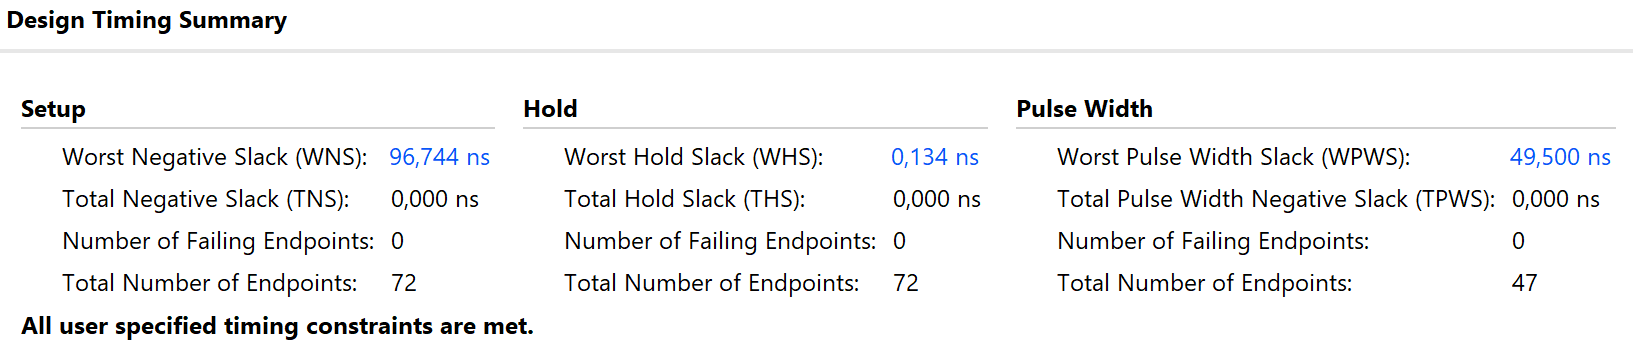
\includegraphics[width=\textwidth]{timing}
    \caption{Report timing del componente sintetizzato.}
    \label{fig:time}
\end{figure}

\subsection{Simulazioni}
Sono stati creati dei test bench per testare il corretto funzionamento del componente secondo le specifiche anche nei casi limite. Il componente passa tutti i test sia in Behavioral Simulation che in Post-Synthesis Functional Simulation.

\subsubsection{Test Bench 1: Sequenza minima e massima}
Il componente si comporta correttamente anche per la codifica di sequenza minima e massima.\\
Nel caso della sequenza minima viene scritto zero all'indirizzo \verb|0x0000|. In questo modo il componente, come in Figura \ref{fig:seq_min}, dopo aver letto che il numero di parole da elaborare è zero, alza il segnale \verb|o_done| e termina la codifica.\\
Nel caso di sequenza massima viene inserito 255 all'indirizzo \verb|0x0000|. Come mostrato in Figura \ref{fig:seq_max}, il componente riesce a codificare tutte le parole compresa l'ultima.

\begin{figure}[ht]
    \centering
    \begin{minipage}{.45\textwidth}
        \centering
        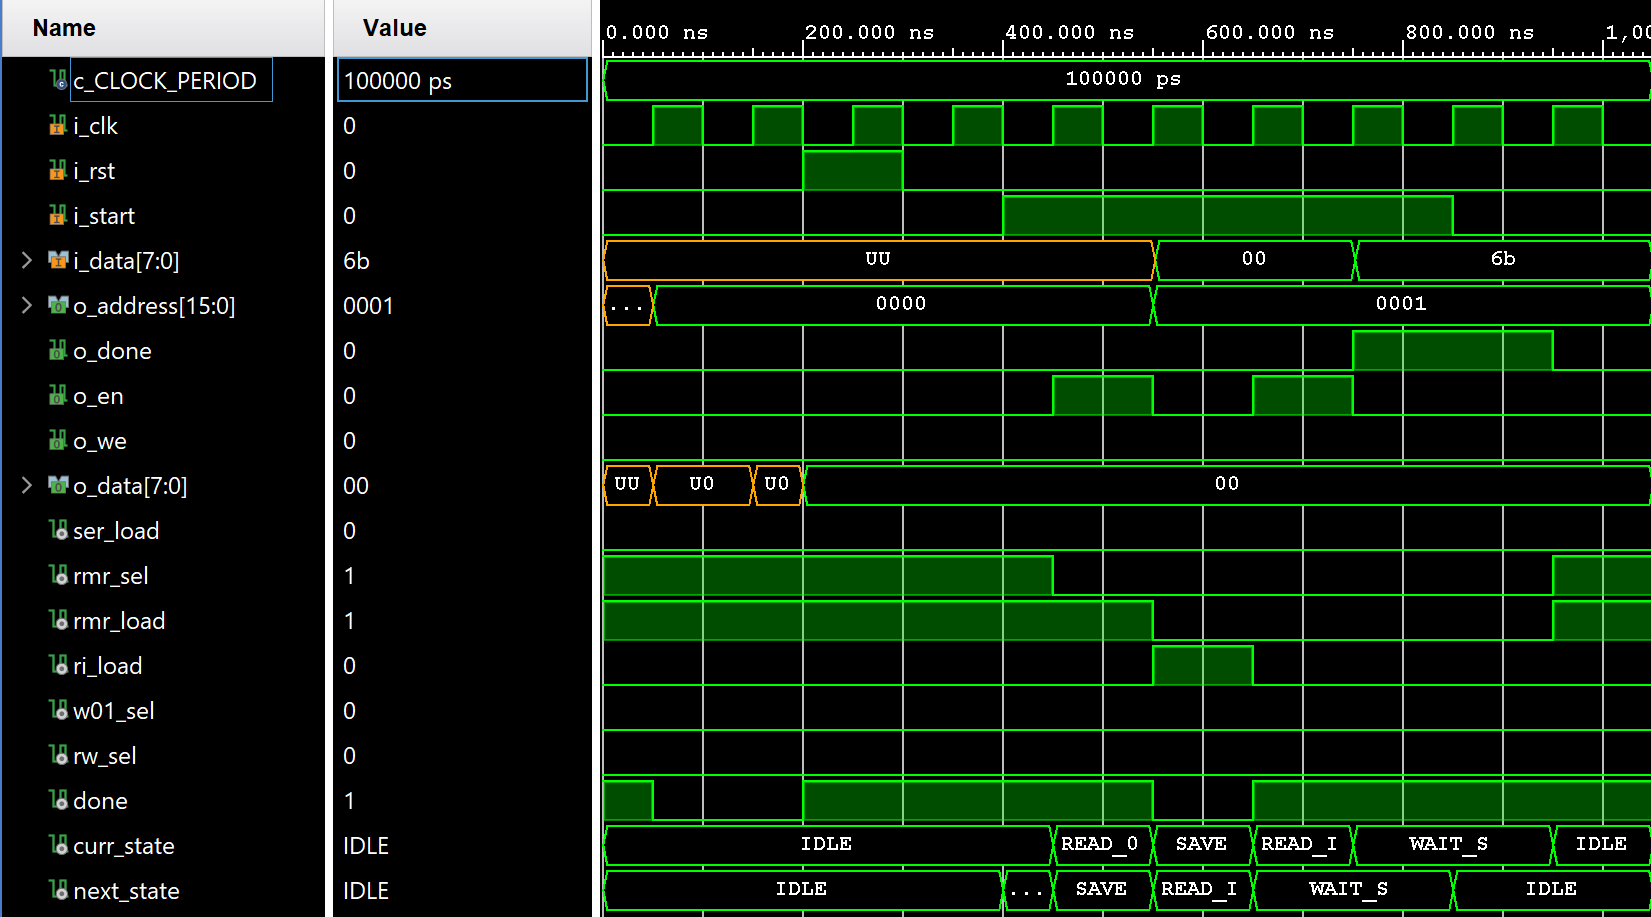
\includegraphics[width=\textwidth]{seq_min}
        \caption{Simulazione test bench 1: sequenza minima.}
        \label{fig:seq_min}
    \end{minipage}
    \hfill
    \begin{minipage}{.45\textwidth}
        \centering
        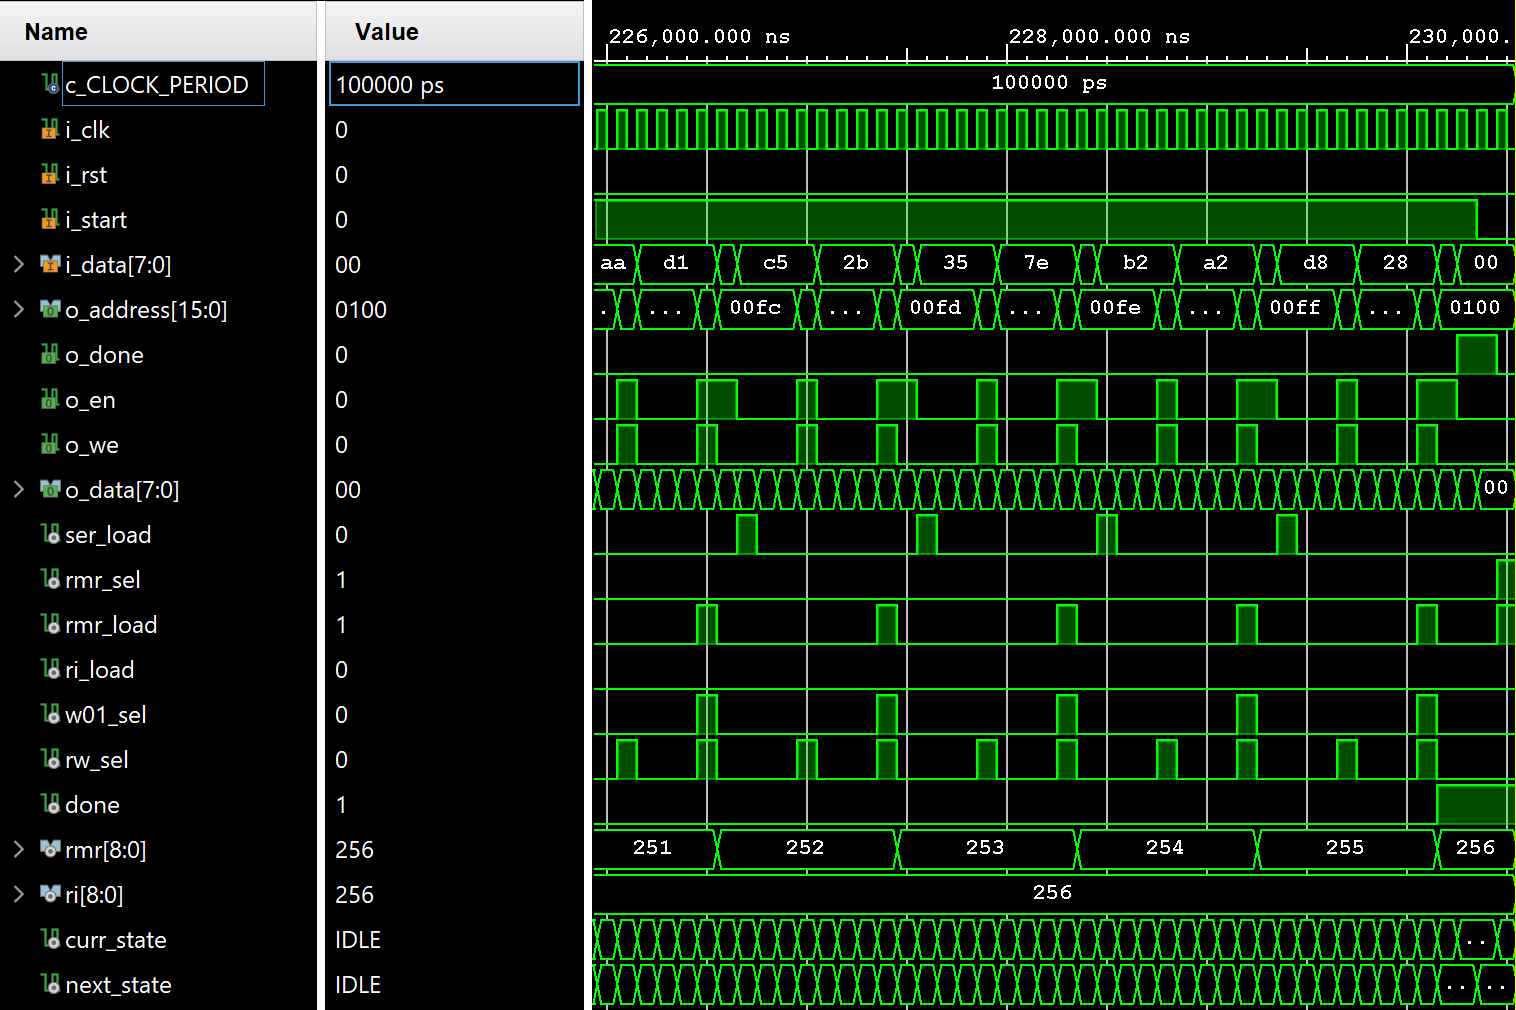
\includegraphics[width=\textwidth]{seq_max}
        \caption{Simulazione test bench 1: sequenza massima (solo parte finale).}
        \label{fig:seq_max}
    \end{minipage}
\end{figure}
\pagebreak
\subsubsection{Test Bench 2: Reset}
Il componente riceve durante la codifica un segnale di reset e, come in Figura \ref{fig:reset}, riesce a ricominciare la codifica correttamente dopo aver ricevuto un nuovo segnale di start.

\begin{figure}[h]
    \centering
    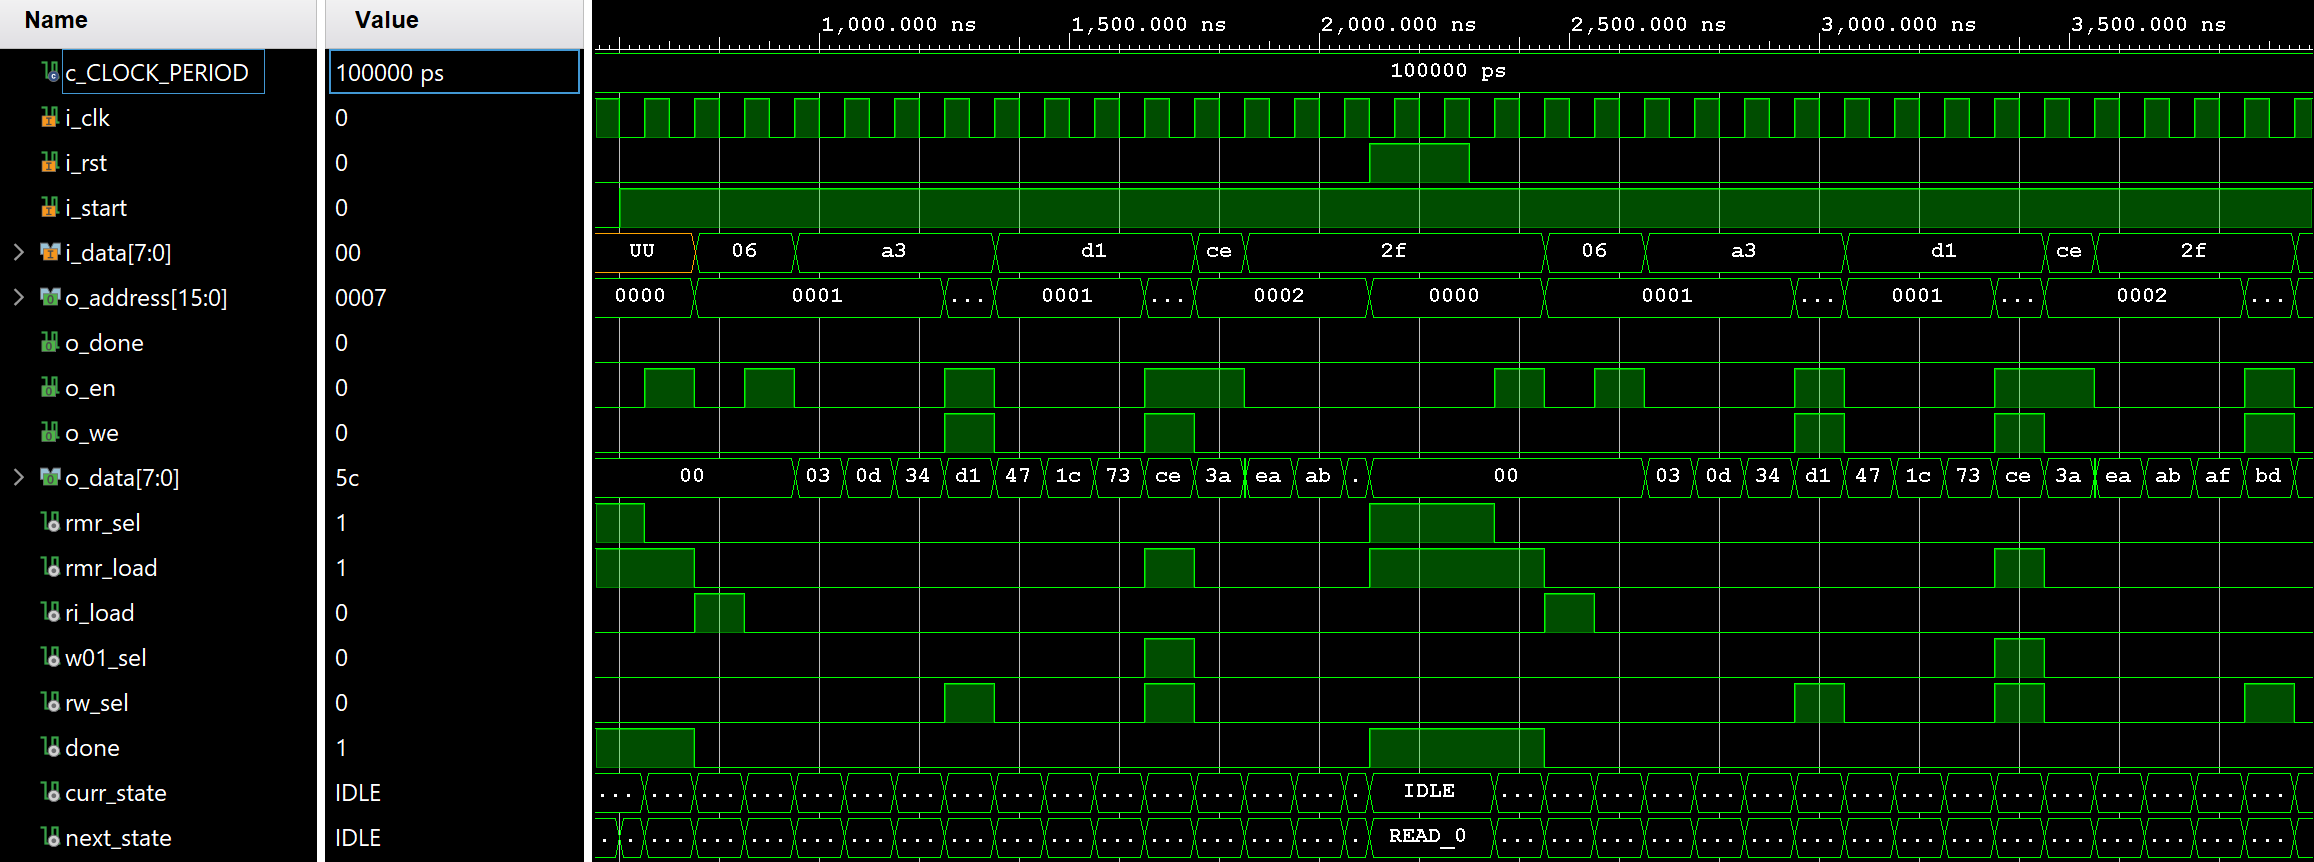
\includegraphics[width=\textwidth]{reset}
    \caption{Simulazione test bench 2: reset.}
    \label{fig:reset}
\end{figure}

\subsubsection{Test Bench 3: Codifica continua}
In questo test bench viene testata la capacità del componente di codificare più sequenze senza ricevere un reset. Come mostrato in Figura \ref{fig:seq_cont}, il componente una volta terminata una sequenza riesce a iniziare correttamente la codifica di una nuova dopo aver ricevuto un nuovo segnale di start.

\begin{figure}
    \centering
    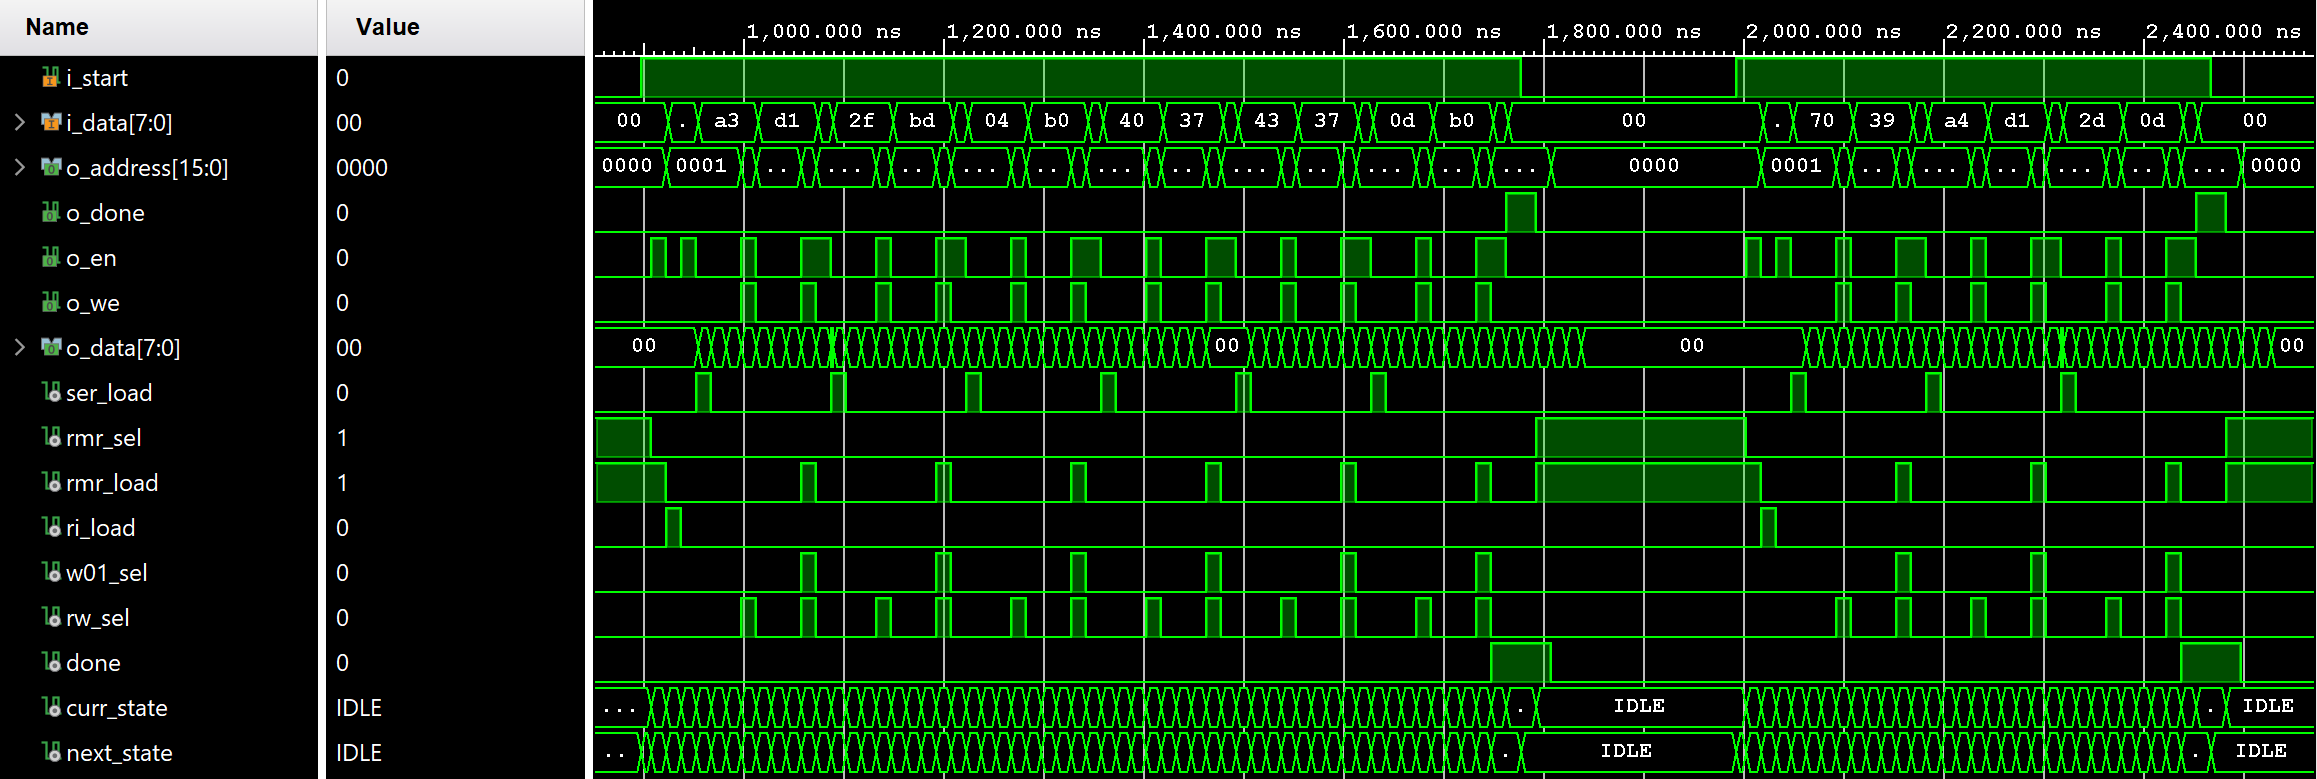
\includegraphics[width=\textwidth]{seq_cont}
    \caption{Simulazione test bench 3: codifica continua.}
    \label{fig:seq_cont}
\end{figure}

\subsubsection{Test Bench 4: Stress Test}
Il componente viene sottoposto ad uno stress test facendogli codificare 10000 sequenze di dimensione variabile tra 0 e 255, rispettivamente minimo e massimo di parole codificabili dal componente in una singola sequenza.\\
Questo test bench ha portato alla scoperta di un errore nella gestione del segnale \verb|o_done|. Inizialmente \verb|o_done| veniva collegato direttamente al segnale \verb|done|, però questo lo portava in rari casi ad alzarsi erroneamente mentre la codifica era ancora in corso. È stato possibile risolvere questo problema semplicemente separando i due segnali e facendo in modo che fosse la macchina a stati a modificare \verb|o_done|.

\section{Conclusioni}
Si ritiene che l'architettura del componente che è stata progettata rispetti pienamente le specifiche. Ciò è stato verificato e confermato dai vari test effettuati.
Inoltre l'architettura è stata pensata per diminuire il più possibile l'overhead alla codifica utilizzando il minimo numero di stati possibili e per minimizzare l'utilizzo di risorse.
Infine il componente è stato suddiviso in più moduli per rendere più semplice la sua progettazione e per facilitare l'identificazione e correzione degli errori.

\end{document}
